\documentclass[a4paper]{article}


\usepackage{alphabeta} 
\usepackage{enumitem} 
\usepackage{mathtools}
\usepackage{amsmath, amssymb} 
\usepackage{amsthm}
\usepackage{cancel} 
\usepackage[margin=0.70in]{geometry} 
\geometry{left=3cm,right=3cm,top=2.4cm,bottom=2.4cm}	%the page geometry as defined, A4=210x297mm
\usepackage{graphicx}
\usepackage{wrapfig}
\usepackage{caption}
\usepackage{textcomp}
\usepackage{tabto}
\usepackage{layout}
\usepackage{bm}
\usepackage{minipage-marginpar}
\usepackage[dvipsnames]{xcolor}
\usepackage{hyperref}
\usepackage{dutchcal}
\usepackage{derivative}
\usepackage{esint}
%\usepackage{biblatex}
\usepackage{subcaption}
\usepackage{booktabs}\usepackage{derivative}
\usepackage[flushleft]{threeparttable}
\usepackage[capbesideposition=outside,capbesidesep=quad]{floatrow}
\usepackage{derivative}
\usepackage[thinc]{esdiff}
%%RENEW

\newtheorem{problem}{Άσκηση}
\newtheorem*{solution*}{Λύση}
\newtheorem{definition}{Ορισμός}[subsection]
\newtheorem{properties}{Ιδιότητες}[subsection]
\newtheorem{theorem}{Θεώρημα}[subsection]
\newtheorem{protash}{Πρόταση}[subsection]
\newtheorem{porisma}{Πόρισμα}[subsection]
\newtheorem{lemma}{Λήμμα}[subsection]
\newtheorem*{prooof}{Απόδειξη}
\newtheorem*{notes}{Παρατηρήσεις}
\newtheorem*{note}{Παρατήρηση}
\newtheorem*{app}{Εφαρμογή} 
\newtheorem*{example}{Παράδειγμα}
\newtheorem*{examples}{Παραδείγματα}


\newcommand\numberthis{\addtocounter{equation}{1}\tag{\theequation}}
%\renewcommand{\labelenumi}{\roman{enumi}}
\newcommand{\approxtext}[1]{\ensuremath{\stackrel{\text{#1}}{\approx}}}
\renewcommand{\figurename}{Εικόνα.}
\renewcommand{\tablename}{Πίνακας.}
%\renewcommand\refname{New References Header}
\renewcommand*\contentsname{Περιεχόμενα}
%\DeclareDerivative{\odv}{\mathrm{d}}


\begin{document}
\begin{titlepage}			%makes a title page. Remember to change the author, CID, username and group number to what is appropriate for you!
	\centering
	{\scshape\LARGE Εθνικό Μετσόβιο Πολυτεχνείο\par}
	{\scshape \LARGE Σ.Ε.Μ.Φ.Ε.\par}
	\vspace{1cm}
	{\huge\bfseries Περίθλαση Ηλεκτρονίων \par}
	\vspace{1cm}
	{\Large\itshape Θωμόπουλος Σπύρος\par}		%remember to change these!
	
	%		{\large Group \@group\unskip\strut\par}
	{\large A.M \hfill \\ E-mail spyros.thomop@gmail.com \\}%ge19042@mail.ntua.gr\par		%remember to change these!
	\vspace{1cm}
	{\large Ημερμονηνία Παράδοσης 2/11/2021\par}
\end{titlepage}


\newpage 

\subsection*{Σκοπός}
Ο στόχος της εν λόγω εργαστηριακής άσκησης είναι η επικύρωση της κυματικής φύσης των ηλεκτρονίων κατά de Broglie, μέσω της περίθλασής τους από λεπτό φύλλο πολυκρυσταλλικού γραφίτη. Επίσης θα προσδιοριστούν οι κρυσταλλικές σταθερές του.


\subsection*{Θεωρητικά Στοιχεία}
\subsubsection*{Κυματοσωματιδιακός Δυϊσμός της Υλης}
Ο φυσικός de Broglie εισήγαγε την αρχή του κυματοσωματιδιακού δυϊσμού της ύλης. Γενικά, η ειδοποιός διαφορά των σωματιδίων από τα κύματα είναι ότι τα μεν σωματίδια είναι εντοπισμένα (ακολουθούν ορισμένη και διακριτή τροχιά) και αδιαίρετα \footnote{Αδιαίρετα με την έννοια ότι δεν είναι συνεχή. Μπορούν να είναι είναι σύνθετα, δηλαδή να αποτελούνται από έναν ακέραιο αριθμό υποσωματιδίων.}, ενώ τα δε κύματα είναι διάχυτα στον χώρο, δηλαδή οδεύουν από ένα σημείο σε ένα άλλο απλωμένα στον χώρο, και διαιρετά. Σύμφωνα με αυτή την αρχή, τα υλικά σωματίδια ($e^-,p^+,n^0$ κλπ) έχουν ένα χαρακτηριστικό που τους προσδίδει την σωματιδιακή φύση το οποίο  σχετίζεται με την δομή τους, ότι είναι αδιαίρετα και ένα που τους προσδίδει την κυματική και σχετίζεται με την κίνησή τους, ότι οδεύουν σαν κύμα και όχι σε συγκεκριμένη Κλασική τροχιά. Κατά αυτή τη λογική, κάθε σωματίδιο που έχει ορμή $\textbf{p}$ και ενέργεια $Ε$ αντιστοιχεί σε ένα κύμα με μήκος κύματος $\lambda$ και συχνότητα $f$. Τα εν λόγω μεγέθη συνδέονται με τις παρακάτω σχέσεις 
\begin{align*}\label{1,2}
E&=hf=\hbar \omega \numberthis\\
p&=\frac{h}{\lambda}=\hbar k \numberthis
\end{align*}

Οι κυματικές ιδιότητες των σωματιδίων αναδύονται σε φαινόμενα περίθλασης, όπως αυτό που θα μελετηθεί. Στην άσκησή μας θα ασχοληθούμε συγκεκριμένα με τα ηλεκτρόνια, για τα οποία προκειμένου να εκδηλωθούν τέτοια φαινόμενα θα πρέπει να διέρχονται από πολύ μικρές σχισμές της τάξης του μήκους κύματος de Broglie που τους αντιστοιχεί, δηλαδή $\sim1 \mathring{A}$. Τόσο μικρή απόσταση συναντάται στο κρυσταλλικό πλέγμα των στερεών, μέσω του οποίου θα διέρχονται τα ηλεκτρόνια σχηματίζοντας εν τέλει μία εικόνα περίθλασης.

\subsubsection*{Περίθλαση ηλεκτρονίων}
Όλη η ανάλυση που έχει προηγηθεί περί κυμάτων de Broglie, ιστορικά είχε προταθεί ορμώμενη από τον κυματοσωματιδικό δυϊσμό του φωτός. Ομοίως, η παρακάτω μεθοδος για την ανάδυση της περίθλασης των ηλεκτρονίων είχε πρώτα εφαρμοστεί για την περίθλαση ακτινών Χ μέσω της οποίας ήταν εφικτή η μέτρηση των αποστάσεων των κρυσταλλικών επιπέδων ενός στερεού (κρυσταλλικό επίπεδο είναι κάθε επίπεδο στο εσωτερικό του στερεού στο οποίο είναι καρφιτσωμένα τα άτομά του).

\begin{wrapfigure}{r}{0.4\textwidth}
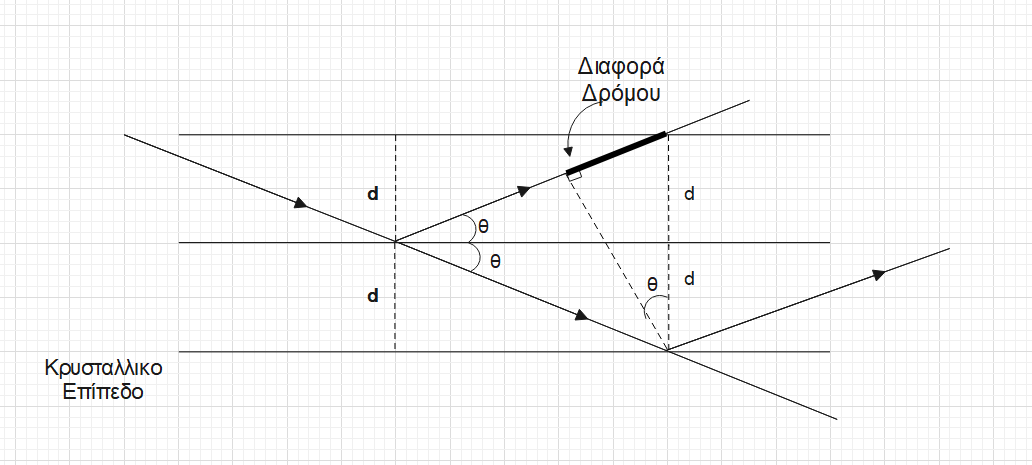
\includegraphics[width=1.3\linewidth]{bragg.png} 
\caption{Σχηματικά το μοντέλο κατά \centering{Bragg}	 }
\label{fig:wrapfig}
\end{wrapfigure}

O Bragg, θεώρησε τα κρυσταλλικά επίπεδο ως ημιπερατά οπτικά κάτοπτρα στα οποία προσπίπτει η ακτινοβολία Χ υπό γωνία $\theta$, η οποία διέρχεται και ανακλάται. Οι ανακλώμενες ακτίνες από τα γειτονικά επίπεδα συμβάλλουν και για να έχουμε ενίσχυση πρέπει να ισχύει η συνθήκη Bragg
\begin{align*}\label{3}
2dsin\theta=m\lambda \numberthis
\end{align*}
όπου $\lambda$ το μήκος κύματος της εισερχόμενης δέσμης, d η απόσταση των διαδοχικών επιπέδων και $m\in \mathbb{N}^*$ η τάξη της περίθλασης. 
Η ίδια ανάλυση γίνεται αν αντικαταστήσουμε τις ακτίνες Χ με ηλεκτρόνια. Επίσης η μέθοδος δουλεύει για μονοχρωματικές ακτίνες Χ και κατ' αντιστοιχία με δέσμη ηλεκτρονίων που έχει μικρή διασπορά $\sim 0.01\%$ στην ταχύτητα.

Στο πείραμα η περίθλαση θα γίνει με την χρήση πολυκρυσταλλικού γραφίτη, ο οποίος αποτελείται λεπτά κρυσταλλικά φύλλα,
\begin{wrapfigure}{r}{0.4\textwidth}
 	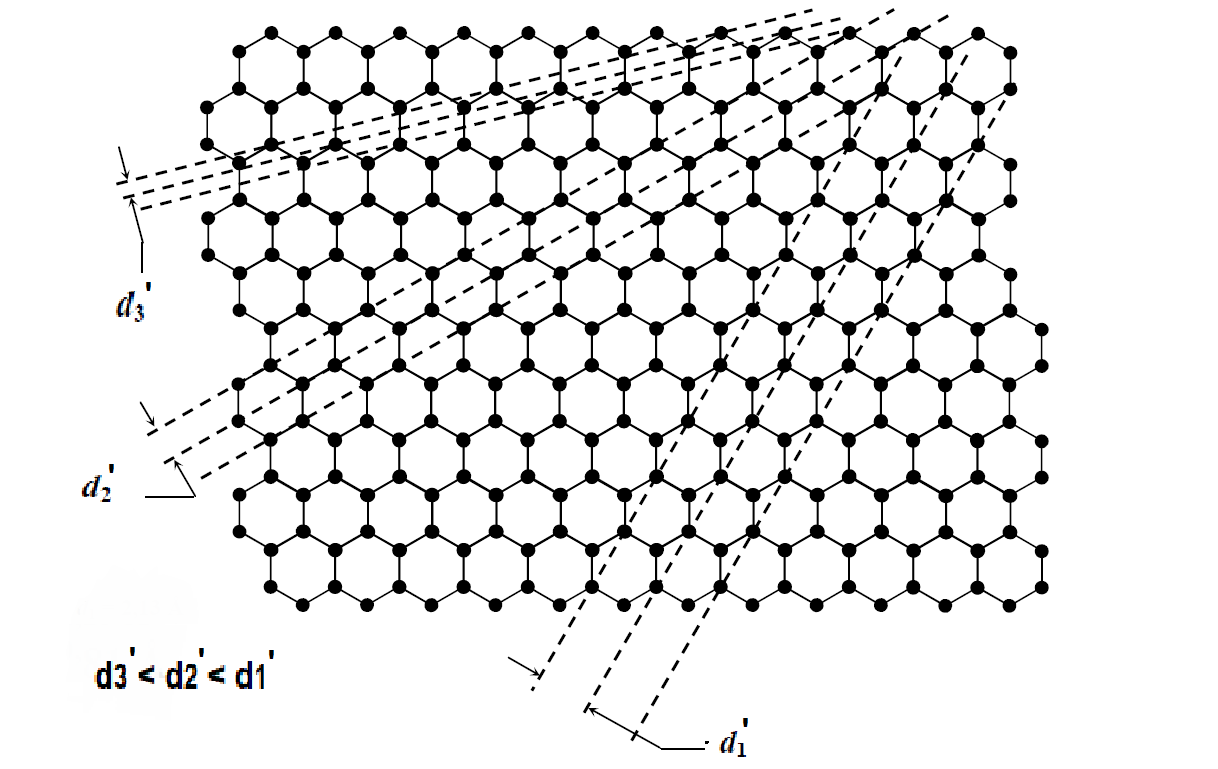
\includegraphics[width=1.0\linewidth]{lattice.png}
 	\caption{ Ατομικό πλέγμα σε φύλλο και χωρική περιοδικότητα} 
 \end{wrapfigure} 	
  τυχαία προσανατολισμένα, πάνω στα οποία κείνται τα άτομα άνθρακα σε κορυφές εξάγωνων κυψελών. 
Σε μία πρώτη σκέψη, η τυχαιότητα του προσανατολισμόυ τους και η έλλειψη χωρικής περιοδικότητας,  οδηγεί στο συμπέρασμα ότι δεν είναι δυνατό να παράξει ενισχυτική συμβολή.
 Ωστόσο, μπορούμε να θεωρήσουμε ως κρυσταλλικό επίπεδο τις ευθείες επί των λεπτών φύλλων οι οποίες ενώνουν τα άτομα άνθρακα, όπως φαίνεται στην Εικόνα 2.
  
 Για τις ευθείες αυτές αλλάζει ο αριθμός ατόμων που βρίσκονται πάνω τους ανα μονάδα μήκους. Η απόσταση δύο διαδοχικών γραμμών ίδιας γραμμικής πυκνότητας σε άτομα είναι σταθερή και ορίζει την περίοδο της εκάστοτε περιοδικότητας. Επομένως η χωρική περιοδικότητα γεννάται από τις ευθείες γραμμές ίδιας πυκνότητας και οι οποίες με την σειρά τους γεννούν την περίθλαση των ηλεκτρονίων.

 Τα επίπεδα-ευθείες γραμμές με την μέγιστη πυκνότητα σε άτομα (οριζόντια με περίοδο $d_1=2.13\mathring{A}$ και κατακόρυφα με περίοδο $d_2=1.23\mathring{A}$ για τον πολυκρυσταλλικό γραφίτη) είναι αυτά από τα οποία παράγεται πίο έντονα η περίθλαση των ηλεκτρονίων και από αυτά θα την μελετήσουμε πειραματικά, ενώ για μικρές πυκνότητες (μικρές χωρικές πείοδοι) δεν ανιχνεύεται περίθλαση.

Πειραματικά, σε μία οθόνη θα ανιχνεύσουμε μία φωτεινή κηλίδα η οποία προκαλείται από τα ηλεκτρόνια τα οποία δεν αλληλεπιδρούν με τον γραφίτη διερχόμενα από το εσωτερικό του. Ακόμη, θα παρατηρήσουμε δύο ομόκεντρους κύκλους, έναν εσωτερικό και εντονότερο τον οποίο προκαλλούν τα ηλεκτρόνια που περιθλώνται από την μεγαλύτερη περιοδικότητα $d_1$ και έναν εξωτερικό και πίο αμυδρό που οφείλεται στην περίθλαση από την μικρή περιοδικότητα $d_2$. Η τάξη της περίθλασης είναι $m=1$. Θα παρατηρηθεί επίσης ένας "θόρυβος" από τα ηλεκτρόνια που χάνουν πολλή ενέργεια από διαδοχικές σκεδάσεις με τα άτομα του γραφίτη.

\subsection*{Πειραματική Διάταξη}
Η πειραματική διάταξη αποτελείται από
\begin{itemize}
\item[.] Λυχνία υψηλού κενού. Η λυχνία με την σειρά της αποτελείται από ένα πυροβόλο ηλεκτρονίων το οποίο λειτουργεί με την θερμιονική εκπομπή ηλεκτρονιών από στρώμα BaO, ένα λεπτό υμένιο από γραφίτη $\sim200\mathring{A}$ και σφαιρική οθόνη στην οποία προσπίπτουν τα ηλεκτρόνια. Η οθόνη είναι επιστρωμένη με τον διάφανο αγωγό $SnCl_2$ ο οποίος απομαρκύνει τα προσπίπτωντα ηλεκτρόνια, που αν συσσωρρεύονταν θα δημιοργούσαν ηλεκτρικό πεδίο ικανό να εκτρέψει ή να επηρεάσει την κίνηση των προσπιπτόντων.
Ακόμη, υπάρχει επίστρωση με την φθορίζουσα ουσία ZnS, η οποία γίνεται πράσινη με την πρόσπτωση των ηλεκτρονίων και μέσω αυτής μπορούμε να παρατηρήσουμε την περίθλαση. Τέλος, για την μέτρηση του τόξου του κύκλου περίθλασης υπάρχει στερεωμένο στην λυχνία ένα υποδεκάμετρο. Η γεωμετρία της λυχνίας φαίνεται στην Εικόνα 3. 
\item[.] Τροφοδοτικό τάσης για την λυχνία
\end{itemize}

\begin{figure}[h!]
\centering
\caption{Λυχνία Κενού }
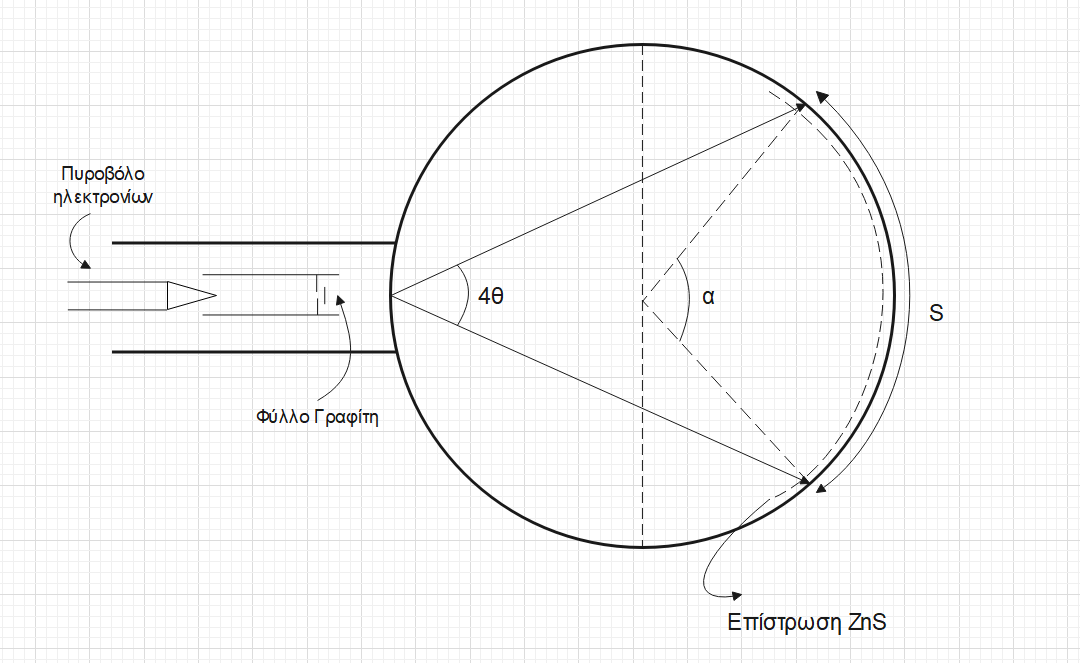
\includegraphics[scale=0.3]{bulb.png}
\end{figure}
Η λυχνία είναι σφαιρική με διάμετρο $D_0=2R_0=(135\pm2)mm$ και s είναι το τόξο του κύκλου περίθλασης που πετράται, άρα ισχύει
\begin{align*}\label{4}
s=\alpha R_0 = 2(4\theta)R_0 = 8\theta D_0/2 \Rightarrow \boxed{\theta =s/4D_0 } \hspace{0.2in} [rad] \numberthis
\end{align*}


\subsection*{Πειραματική Διαδικασία - Επεξεργασία Μετρήσεων}
Ανοίγουμε το τροφοδοτικό και περιμένουμε 2-3 λεπτά ώστε να θερμανθεί η κάθοδος στο πυροβόλο ηλεκτρονίων. Αυξάνουμε την τάση της καθόδου απ'το τροφοδοτικό από $1500-3500V$ με βήμα $500V$ και μετράμε το μήκος του τόξου των δύο κύκλων περίθλασης που δημιουργούνται στην οθόνη, θεωρώντας $s_1$ τον μικρό και $s_2$ τον μεγάλο. Έπειτα επαναλαμβάνουμε τις μετρήσεις για μειούμενη τάση από $3500-1500V$ με βήμα $500V$. \textcolor{red}{Το σφάλμα της τάσης το θεωρούμε $\delta V =0 V$}, ενώ του τόξου $\delta S_i = 0.3cm$.
\\
Το ηλεκτρόνιο κατά την κίνησή του στο κενό δεν θα έχει δυναμική ενέργεια επομένως η ολική του ενέργεια θα είναι κινητική, άρα 
$E=p^2/2m_e\Rightarrow p = \sqrt{2m_eE}$. Την εν λόγω κινητική θα την έχει προσλάβει από την εφαρμογή του δυναμικού V στη κάθοδο του τηλεβόλου, άρα $E=eV$ και από την σχέση (2) έχουμε ότι
\begin{align*}\label{5}
\lambda = \frac{h}{p}  = \frac{h}{\sqrt{2m_eE}} = \frac{h}{\sqrt{2m_e eV}} \simeq \frac{12.25}{\sqrt{V}}\mathring{A} \numberthis
\end{align*}
Έτσι από τις μετρήσεις μας και την σχέση (\ref{5}) συμπληρώνουμε τον Πίνακα 1, όπου $\overline{s_i}$ η μέση τιμή του μήκους του τόξου για τις δύο περιπτώσεις μετρήσεων (αυξανόμενη και μειούμενη τάση). 

\begin{table}[h!]
\centering
\caption{ }
\begin{tabular}{r|r|r|r|r|r|r|r|r}
\textcolor{red}{$V_i( V)$} & $\sqrt{V_i}$ & $\lambda_i(\mathring{A})$ & \multicolumn{2}{r|}{$s_1(\pm0.3cm)$} & 							\textcolor{red}{$\overline{s_1}(cm)$}&\multicolumn{2}{r|}{$s_2(\pm0.3cm)$} & \textcolor{red}{$\overline{s_2}(cm)$} \\
\hline\hline 
%1.5000& 0.0387& 0.0003&  0.0041& 0.0038& 0.0070& 0.0070\\
%2.0000& 0.0447& 0.0003&  0.0032& 0.0035& 0.0063& 0.0061\\
%2.5000& 0.0500& 0.0002&  0.0029& 0.0031& 0.0052& 0.0054\\
%3.0000& 0.0548& 0.0002&  0.0028& 0.0028& 0.0049& 0.0050\\
%3.5000& 0.0592& 0.0002&  0.0027& 0.0027& 0.0047& 0.0047

1500&38.73&0.32&4.1&3.8&3.95&7.0&7.0&7.00\\
2000&44.72&0.27&3.2&3.5&3.35&6.3&6.1&6.15\\
2500&50.00&0.25&2.9&3.1&3.00&5.2&5.4&5.30\\
3000&54.77&0.22&2.8&2.8&2.80&4.9&5.0&4.95\\
3500&59.16&0.21&$\underbrace{2.7}_{\uparrow}$&$\underbrace{2.7}_{\downarrow}$&2.70&$\underbrace{4.7}_{\uparrow}$&$\underbrace{4.7}_{\downarrow}$ &4.70
\end{tabular}
\end{table}
Ακόμη, από την σχέση (\ref{3}) του Bragg για τάξη περίθλασης $m=1$ και την σχέση (\ref{5}) παίρνουμε για την σταθερά του πλέγματος
\begin{align*}\label{6}
d \sqrt{V}= \frac{6.125}{sin\theta}  \hspace{0.3in} [\mathring{A}] \numberthis
\end{align*} 

Από την σχέση (\ref{4}), προκειμένου να εκμεταλλευτούμε την σχέση (\ref{6}), προκύπτει ο παρακάτω πίνακας
\begin{table}[h!] 
\centering
\caption{ }
\begin{tabular}{r|r|r|r|r|r|r|r|r}
$\sqrt{V_i}$ & $\overline{s_1}(cm)$&$\overline{s_2}(cm)$&$\theta_1(rad)$&$\theta_2(rad)$&$sin\theta_1$&$sin\theta_2$&$6.125/sin\theta_1$&$6.125/sin\theta_2$ \\
\hline\hline
38.73&4.0&7.0&0.073&0.130&0.073&0.130&83.81&47.38\\
44.72&3.4&6.2&0.062&0.114&0.062&0.114&98.80&53.90\\
50.00&3.0&5.3&0.056&0.098&0.056&0.098&110.31&62.51\\
54.77&2.8&5.0&0.052&0.092&0.052&0.092&118.18&66.91\\
59.16&2.7&4.7&0.050&0.087&0.050&0.087&122.55&70.46\\
\end{tabular}
\end{table}

Θέτουμε $Y=6.125/sin\theta_i$ και $X=\sqrt{V}$ και τότε η σχέση (\ref{6}) γίνεται $Y=d_iX$, για $i=1,2$.
Εφαρμόζουμε δύο φορές την μέθοδο ελαχίστων τετραγώνων για τις στήλες 1-8 και 1-9, απαιτώντας για τις ευθείες μας να περνάνε από την αρχή των αξόνων, δηλαδή να είναι της μορφής $Y=A_i X$.\footnotemark
\footnotetext{Η κλίση για την ευθεία $Y=AX$ που προσαρμόζεται βέλιστα στα δεδομένα $(x_i,y_i)$ δίνεται από την σχέση $A=\frac{\sum_{i=1}^{n}x_iy_i}{\sum_{i=1}^{n}x_i^2}$ και το αντίστοιχο σφάλμα $(\delta A)^2=\sigma_A^2=
\frac{\sigma_y^2}{\sum_{i=1}^{n}x_i^2}$, όπου
 $\sigma_y\simeq\sum_{i=1}^{n}\frac{(y_i-bx_i)^2}{n-1}$.}
 Τότε, θα προκύψουν οι αποστάσεις των κρυσταλλικών επιπέδων που έχουν την μεγαλύτερη πυκνότητα σε άτομα (οριζόντια και κάτακόρυφα)  $d_1$ και $d_2$, ως οι κλίσεις των εν λόγω ευθειών ελαχίστων τετραγώνων:
\begin{align*}
d_1 = (2.15\pm0.03)\mathring{A} \\
d_2 = (1.23\pm0.01)\mathring{A}
\end{align*}
Στην Εικόνα 4 φαίνονται και οι αντίστοιχες γραφικές παραστάσεις.

\begin{figure}[h!]
\centering
\caption{Πειραματικά Δεδομένα - Ευθείες Ελαχίστων Τετραγώνων  (διερχ. από αρχή των αξόνων)}
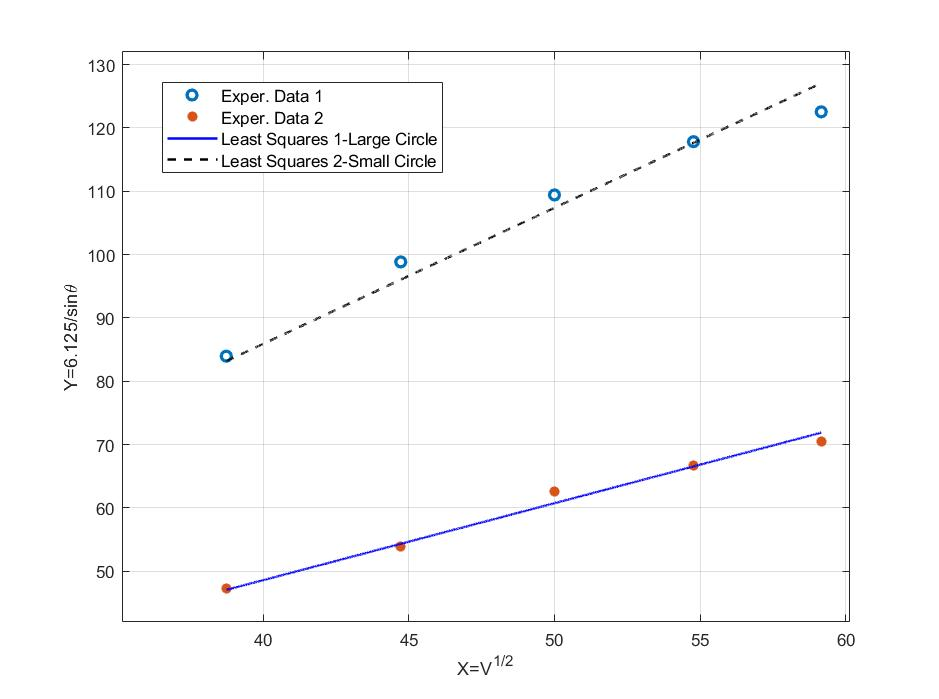
\includegraphics[scale=0.5]{leastsq.jpg}
\end{figure}

\subsection*{Συμπεράσματα}
Παρατηρούμε ότι οι τιμές των αποστάσεων των κρυσταλλικών επιπέδων που υπολογίστηκαν πειραματικά συμπίπτουν με τις θεωρητικές που αναμέναμε, συνεπώς η συνολική διαδικασία.
\subsection*{Βιβλιογραφία}
\begin{itemize}
\item[.]  Εργαστηριακές Ασκήσεις Φυσικής, ΤΟΜΟΣ Ι, ΣΥΛΛΟΓΙΚΟ
\item[.]  Εργαστηριακές Ασκήσεις Φυσικής, ΤΟΜΟΣ ΙI, ΣΥΛΛΟΓΙΚΟ
\end{itemize}

\end{document}